\documentclass[dvisvgm,tikz,margin=2pt]{standalone}
\usepackage{amsmath,amssymb,amsthm}
\usepackage{tikz}
\usetikzlibrary{patterns}
\usepackage{xcolor}
\newcommand{\R}{\mathbb{R}}
\newcommand{\vol}{\operatorname{vol}}
\newcommand{\HV}{\operatorname{HV}}
\newcommand{\Oh}{\mathcal{O}}
\begin{document}
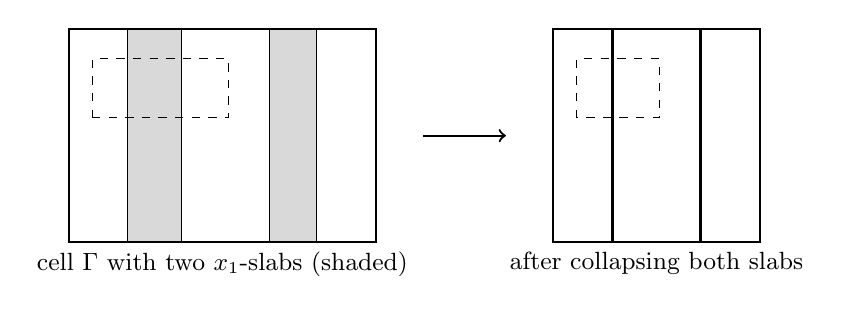
\begin{tikzpicture}[scale=1.5]
  % left: cell with two slabs
  \begin{scope}
    \draw[thick] (0,0) rectangle (2.6,1.8);
    \fill[black!15] (0.5,0) rectangle (0.95,1.8);
    \fill[black!15] (1.7,0) rectangle (2.1,1.8);
    \draw (0.5,0) rectangle (0.95,1.8);
    \draw (1.7,0) rectangle (2.1,1.8);
    \draw[dashed] (0.2,1.05) rectangle (1.35,1.55);
    \node[below] at (1.3,0) {\small cell $\Gamma$ with two $x_1$-slabs (shaded)};
  \end{scope}
  \draw[->,thick] (3.0,0.9) -- (3.7,0.9);
  % right: collapsed
  \begin{scope}[xshift=4.1cm]
    \draw[thick] (0,0) rectangle (1.75,1.8);
    \draw[very thick] (0.5,0) -- (0.5,1.8);
    \draw[very thick] (1.25,0) -- (1.25,1.8);
    \draw[dashed] (0.2,1.05) rectangle (0.9,1.55);
    \node[below] at (0.875,0) {\small after collapsing both slabs};
  \end{scope}
\end{tikzpicture}
\end{document}
